\providecommand{\main}{..}
\documentclass[\main/main.tex]{subfiles}

\begin{document}
\graphicspath{{img/}{04_hardware/img/}}

\chapter{Anchor hardware implementation}

\section{Introduction to DWM1001 module}
\begin{figure}[H]
    \begin{center}
        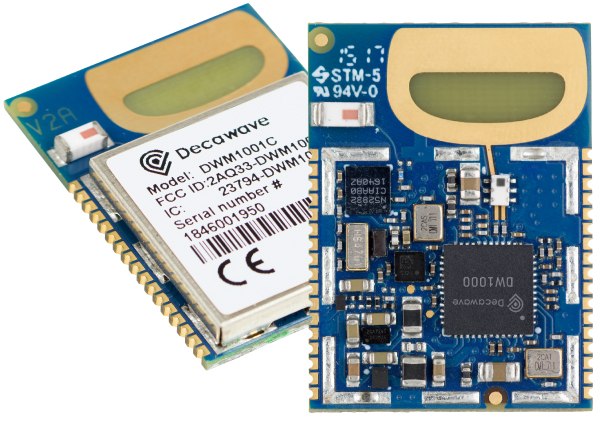
\includegraphics[scale=0.35]{DWM1001-Module_ProdPage_600x430.jpg}
    \end{center}
    \caption{DWM1001 Module}
    \label{fig:dwm1001c_module}
\end{figure}

The DWM1001 module is based on Decawave's DW1000 Ultra
Wideband (UWB) transceiver IC, which is an IEEE 802.15.4-
2011 UWB implementation. It integrates UWB and Bluetooth
antenna, all RF circuitry, Nordic Semiconductor nRF52832 and
a motion sensor.

There are multiple reasons for answering the question why DWM1001 module is used for this thesis.
Followings are some key features:
\begin{itemize}
    \item Ranging accuracy to within 10cm
    \item UWB Channel 5 printed PCB antenna (6.5 GHz)
    \item 6.8 Mbps data rate IEEE 802.15.4-2011 UWB compliant
    \item Well known Nordic Semiconductor nRF52832 SoC
    \item Bluetooth connectivity and Bluetooth chip antenna
    \item Motion sensor is available: 3-axis accelerometer
    \item Current consumption optimized for low power sleep mode: $<$ 15$\mu$A
    \item Low supply voltage: 2.8 V to 3.6 V
    \item Small size: 19.1 mm x 26.2 mm x 2.6 mm
    \item Modules marked DWM1001C are certified to ETSI, FCC and ISED regulations
\end{itemize}

\begin{figure}[H]
    \begin{center}
        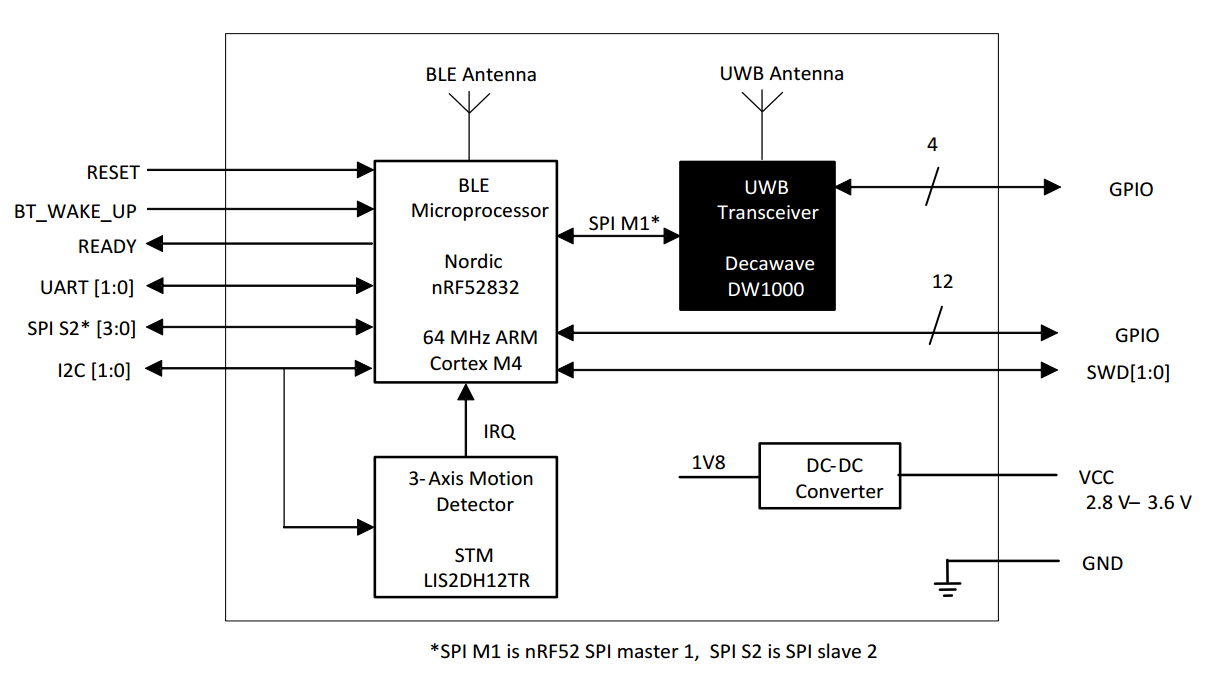
\includegraphics[scale=0.35]{dwm1001_block_diagram.png}
    \end{center}
    \caption{DWM1001 block diagram}
    \label{fig:dwm1001_block_diagram}
\end{figure}

The nRF52832 is a general-purpose multi-protocol SoC. It meets the challenges of a broad range of applications that need advanced Bluetooth LE features. It is built around an Arm® Cortex™-M4 CPU with floating-point unit running at 64 MHz. In the DWM1001 module, it communicates with DW1000 radio IC over a SPI connection.

\section{Battery charger circuit}

\begin{figure}[H]
    \begin{center}
        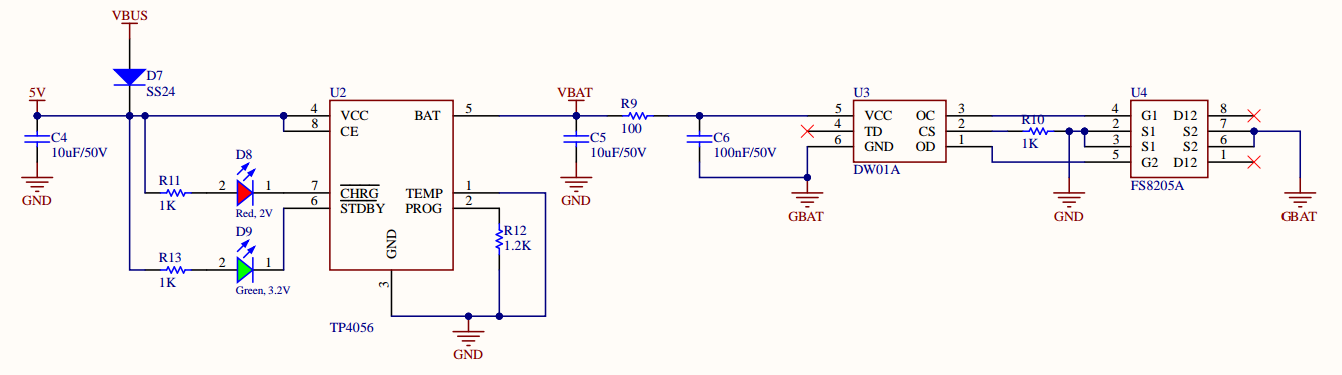
\includegraphics[scale=0.35]{battery_charger_circuit.png}
    \end{center}
    \caption{Battery charger circuit}
    \label{fig:battery_charger_circuit}
\end{figure}

\subsection{TP4056}

\subsection{DW01A and FS8205A}

\section{Voltage step down converter}
\begin{figure}[H]
    \begin{center}
        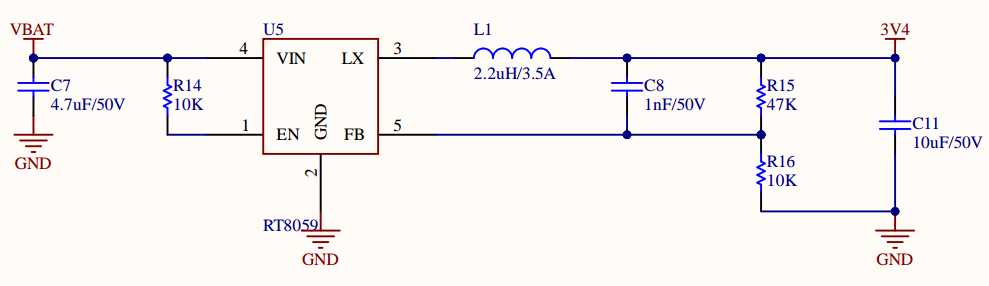
\includegraphics[scale=0.5]{voltage_set_down_converter.png}
    \end{center}
    \caption{Voltage set down converter}
    \label{fig:voltage_set_down_converter}
\end{figure}

\section{220V Solid State Relay}
\begin{figure}[H]
    \begin{center}
        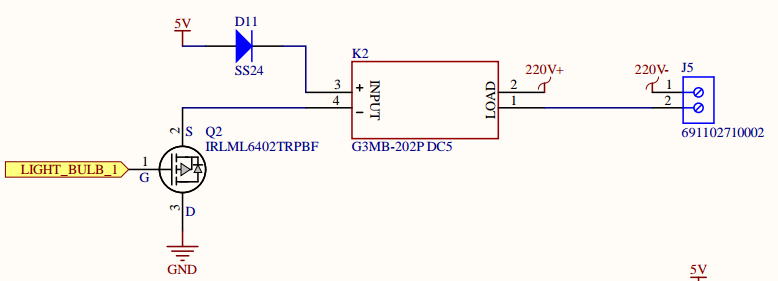
\includegraphics[scale=0.5]{relay_circuit.png}
    \end{center}
    \caption{Relay circuit}
    \label{fig:relay_circuit}
\end{figure}

\end{document}